%!TEX TS-program = xelatex
\documentclass[]{friggeri-cv}
\usepackage{afterpage}
\usepackage{hyperref}
\usepackage{color}
\usepackage{xcolor}
\usepackage{fontspec}
\usepackage[utf8]{inputenc}
\usepackage{enumitem}

\hypersetup{
    pdftitle={Wesley Banfield CV},
    pdfauthor={Wesley Banfield},
    pdfsubject={CV},
    pdfkeywords={CV Wesley Banfield},
    colorlinks=false,
    allbordercolors=white
}

\RequirePackage{xcolor}
\definecolor{pblue}{HTML}{0395DE}

\begin{document}

\begin{figure}[!h]
	\begin{minipage}{0.48\textwidth}
		\begin{flushleft}
			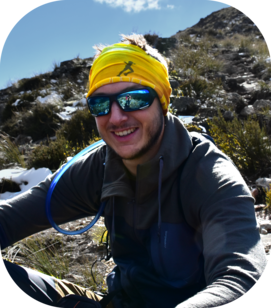
\includegraphics[width=2.75cm]{img/profile_relaxed_compressed.png}
		\end{flushleft}
	\end{minipage}\hfill
	\header{Wesley}{ Banfield}
 	{Senior Software Engineer - Geoscience Platforms}
	\begin{minipage}{0.48\textwidth}
		\begin{flushright}
			
\includegraphics[width=2.75cm]{img/qrcode.png}
		\end{flushright}
	\end{minipage}
\end{figure}
\vspace{-0.75cm}
% Fake text to add separator      
\fcolorbox{white}{gray}{\parbox{\dimexpr\textwidth-2\fboxsep-2\fboxrule}{%
.....
}}

\begin{quote}
\large
\begin{center}
Senior software engineer with proven expertise in R\&D, platform development, and technical leadership across climate science and natural resources sectors.
\\
\end{center}
\end{quote}

\begin{center}
\vspace{6pt}
\href{mailto:wesleybanfield@gmail.com}{\textbf{wesleybanfield@gmail.com}}
\vspace{3pt}
\\+33 7 52 08 02 37, Albertville, France
\vspace{3pt}
\\\emph{GB / USA citizen, FR bilingual}
\vspace{3pt}
\\\href{https://www.linkedin.com/in/wesleybanfield/}{LinkedIn},
\href{https://github.com/WesleyTheGeolien}{GitHub},
\href{https://wesleythegeolien.github.io}{Website}
\end{center}

\vspace{18pt}
\section{Skills}
\begin{itemize} 
	\item {\large\textbf{\textcolor{pblue}{Languages \& Frameworks}}}: Python, Docker, TypeScript, React, C++, SQL, Latex
	\item {\large\textbf{\textcolor{pblue}{Cloud \& Infrastructure}}}: APIs, Serverless Compute, Micro Services
	\item {\large\textbf{\textcolor{pblue}{Specialization}}}: Scientific Computing, Data Visualization, Generative AI
	\item {\large\textbf{\textcolor{pblue}{Technical Leadership}}}: Prototyping, Stakeholder Communication, Cross-functional Collaboration, Innovation
\end{itemize}
\vspace{1em}

\section{Experience}
\begin{entrylist}
	
	\entry
	{8/21 - Now}
	{Senior Full Stack Developer}
	{\href{https://resourcemodelingsolutions.com/}{Resource Modeling Solutions, Remote}}
	{
	Develop and maintain industry-standard geostatistical Python package (rmsp) and platform with state-of-the-art functionality for Breakthrough Energy-backed organization.
	\\[-0.5em]
	\begin{itemize}[label={}, itemsep=3pt, leftmargin=0pt]
		\item \textbf{AI Integration:} Implemented cloud-based assistant using LLMs with RAG capabilities, providing contextualized code suggestions and documentation searches grounded in proprietary geological data
		\item \textbf{3D Visualization:} Built and maintain interactive 3D geological data viewer integrated into Jupyter notebooks using vtk.js, with custom data conversion pipelines
		\item \textbf{DevOps Leadership:} Spearheaded comprehensive testing framework implementation, orchestrated Git LFS migration for large asset management, and integrated code coverage analysis into CI pipelines
		\item \textbf{Platform Integrations:} Led integration of C libraries into Python package and prototyped workflows between rmsp and GeologicAI's Coretable for enhanced geological modeling
		\item \textbf{Web Development:} Developed company website from mock ups.
		\item \textbf{Development Operations:} Managed feature development, bug fixes, client support, and code reviews for production geological modeling platform
	\end{itemize}
	}

	\entry
	{2023}
	{Team Lead Tech and Infrastructure (Volunteer)}
	{\href{https://sites.google.com/climatematch.io/academy/about}{Climatematch, Remote}}
	{
		Led technical infrastructure for globally accessible climate science summer school program, democratizing access to computational methods in climate science for diverse international community.
		\\[-0.5em]
		\begin{itemize}[label={}, itemsep=3pt, leftmargin=0pt]
			\item \textbf{DevOps Leadership:} Oversaw development of GitHub Actions pipelines for automated code testing and Jupyter Book creation, ensuring reliable content delivery
			\item \textbf{Environment Management:} Curated unified computational environment based on Pangeo stack, providing students with comprehensive toolset for climate science coursework
			\item \textbf{Infrastructure Coordination:} Served as primary liaison with 2i2c for JupyterHub setup and maintenance, ensuring seamless learning platform for global participants
		\end{itemize}
	}
  \end{entrylist}
  \vspace*{\fill}
\newpage
\vspace*{\fill}
\begin{entrylist}
	\entry
	{9/20 - 7/21}
	{Research Engineer - Climate}
	{\href{https://paleoclim-cnrs.github.io/}{Protisvalor - CEREGE, France}}
	{
	Collaborated with paleoclimatology workgroup within leading French geosciences research center, working closely with researchers across France and Europe on computational climate science initiatives.
	\\[-0.5em]
	\begin{itemize}[label={}, itemsep=3pt, leftmargin=0pt]
		\item \textbf{SaaS Platform Development:} Developed, deployed, and maintained Software as a Service platform for IPSL climate model boundary condition configuration, enhancing usability through interactive input construction and open-sourced on GitHub
		\item \textbf{Data Processing Pipeline:} Contributed to development of semi-automated processing pipeline for climate data analysis, successfully deployed on internal JupyterHub instance under my management
		\item \textbf{Technical Infrastructure:} Managed JupyterHub deployment, facilitating efficient and streamlined data processing workflows for research team
		\item \textbf{Community Engagement:} Actively engaged with Pangeo group to advance understanding of computational climate science best practices and methodologies
	\end{itemize}
	}
 	\entry
	{10/19 - 6/20}
	{Project Manager Digital Innovation}
	{\href{http://envisol.net/}{Envisol, France}}
	{
	Led digital innovation initiatives at French consultancy specializing in contamination and remediation, driving technological advancement in environmental assessment workflows.
	\\[-0.5em]
	\begin{itemize}[label={}, itemsep=3pt, leftmargin=0pt]
		\item \textbf{SaaS Platform Development:} Constructed prototype geostatistical Software as a Service solution for contamination characterization, leveraging advanced geostatistical techniques to provide detailed contamination level insights
		\item \textbf{Decision Support Systems:} Designed solution to accurately characterize and regularly update contamination estimates, supporting informed decision-making and remediation strategies
		\item \textbf{Workflow Automation:} Automated data acquisition workflows, streamlining environmental data collection and processing procedures
		\item \textbf{QGIS Development:} Built bespoke tools for QGIS platform, enhancing geospatial analysis capabilities for contamination assessment projects
	\end{itemize}
	}
  
 	\entry
    {01/17 - 05/19}
    {Research Engineer}
    {\href{https://www.seequent.com/}{Seequent, New Zealand}}
    {
	Contributed to R\&D team at leading geological modeling software company, recognized for creating Leapfrog 3D suite utilizing Radial Basis Functions (RBFs) to generate surfaces from sparse geological input data.
    \\[-0.5em]
   	\begin{itemize}[label={}, itemsep=3pt, leftmargin=0pt]
		\item \textbf{Geostatistical Validation:} Validated internal geostatistical implementations, ensuring scientific accuracy and robustness for Leapfrog EDGE
		\item \textbf{Cross-functional Collaboration:} Collaborated with internal teams and clients to deliver technical expertise and innovative geological modeling solutions, bridging R\&D capabilities with market needs
		\item \textbf{Rapid Prototyping:} Developed prototypes by repurposing existing Core IP and exploring innovative approaches including cloud-based computations and web dashboards for geological applications
		\item \textbf{User-Centric Development:} Implemented iterative design processes to gather valuable user feedback, refining and enhancing solutions to deliver high-quality, user-focused geological modeling tools
	\end{itemize}
    % \\
    % Reference : \href{mailto:tim.schurr@seequent.com}{Tim Schurr, Solutions Architect}
	}
  
	% \entry
    % {05/16 - 09/16}
    % {Software Integration Engineering Internship}
    % {\href{https://www.total.com/en}{Total, Pau France}}
    % {Discretization plays an important part in coupled Oil \& Gas basin modelling. Too fine, the computation time prevails, too coarse and the calculations do not converge. As a software integration engineer I implemented an interface with the \href{http://www.ring-team.org/software/ringmesh}{RINGMesh} library to dynamically re-mesh during simulations.\\ Reference : \href{mailto:tristan.cornu@total.com}{Tristan Cornu, Pore pressure and Rock Mechanics Specialist}}

    % \entry
    % {02/16 - 05/16}
    % {Research Intern}
    % {\href{http://www.ring-team.org/}{Ring Research Lab, Nancy France }}
    % {Research and implementation of different automatic simultaneous well log correlation algorithms and creation of a SKUA-Gocad plug-in. The master's thesis was carried out in the lab that originally developed SKUA-Gocad before commercialisation by Paradigm. The work was presented and published in the 2016 Ring Meeting. \\Reference : \href{mailto:Guillaume.Caumon@ensg.univ-lorraine.fr}{Dr. Guillaume Caumon, Head of Research team}}
    
	% \entry
    % {06/15 - 09/15}
    % {Software Engineering Internship}
    % {\href{https://www.seequent.com/}{Seequent, Christchurch New Zealand}}
    % {Design and development of a graphical user interface for geostatistical analysis in Leapfrog 3D Geological modelling suite, later integrated into Leapfrog EDGE. Implementation of different geostatistical algorithms.
    % \\
    % Reference : \href{mailto:tim.mclennan@seequent.com}{Tim McLennan}}

	% \entry
	% {09/14 - 05/15}
	% {Lab Research Project}
	% {\href{http://georessources.univ-lorraine.fr/}{GeoRessources, Nancy France}}
	% {Geochemistry can be used to date oil, however when in contact with water certain couples reset. The goal of the project was to develop an experimental protocol to analyse the behaviour of the Rhenium / Osmium couple. Automated graphing tools where developed to analyse the ICP-MS results.
	% 	\\
	% 	Reference : Raymond Michels}
\end{entrylist}
\vspace*{\fill}
\newpage
\vspace*{\fill}
\section{Presentations and Publications}
\begin{entrylist}
	\entry
	{2021}
	{Reproducible Compute Environments with Docker}
	{Paleoclim France}
	{\href{https://wesleythegeolien.github.io/Presentations/docker_reproducible_envs/index.html}{Presentation to work group how container technology can be harnessed to produce reproducible coding environments for publications and work.}}
	\entry
	{2021}
	{Portable interactive Plotting with Javascript}
	{Software Underground}
	{1h30 talk on how to use Python with Javascript to create portable graphs that can be used in any web browser. Viewable on \href{https://www.youtube.com/watch?v=j\_4wkMzGvKs}{YouTube.}}
	\entry
	{2020}
	{Prototyping for Geologists}
	{Transform 2020}
	{Short talk on building an infrastructure to rapidly build and deploy prototypes.
	Viewable on \href{https://youtu.be/rUbvueIF5f8?t=4130}{YouTube}.}
	\entry
	{2019}
	{JupyterLab Quick Start Guide}
	{Packt}
	{Coauthor of JupyterLab quick start guide.}
	\entry
	{2019}
	{Integration of BIM and the subsurface}
	{Indura Cluster}
	{Presentation demonstrating the integrations between Building Information Modeling and subsurface data.}
	\entry
	{2018}
	{How certain are you of your surfaces}
	{Seequent Lyceum Perth}
	{Presentation in front of over 200 mining experts on behalf of Seequent demonstrating the latest R\&D work carried out at the company. Viewable on \href{https://www.youtube.com/watch?v=jt26J5ljlA0}{YouTube}.}
	\entry
	{2016}
	{Current automatic well log correlation techniques}
	{Ring Consortium}
	{Presentation in front off over 100 Oil and Gas experts demonstrating my Master's thesis on automated well log correlation techniques. The Master's thesis was also published in the Proceedings.}
\end{entrylist}
\section{Open Source Contributions}
\begin{entrylist}
	\entry
	{2021}
	{Seismic Footprint removal Hackathon}
	{Transform 2021}
	{Build a tool to design filters for seismic data in the frequency domain. After the hackathon a web based tool (panel) was built and deployed to AWS.}
	\entry
	{2020 - 2021}
	{Pangeo collaborator}
	{Pangeo}
	{Take part in weekly catchups to discuss and better understand the intersection between computing and climate sciences}
	\entry
	{2020 - 2021}
	{SOS Mediterranée website update}
	{CartONG}
	{Refresh of the website to show boat rescues in the mediterranean sea.}
	\entry
	{2020}
	{Well Correlation tool Hackathon}
	{Transform 2020}
	{Build a web tool (Dash / Plotly) to load LAS files and visualize them.}
\end{entrylist}
\section{Education MEng, MSc}
\begin{entrylist}
  \entry
    {2013 - 2016}
    {Master in Geological Engineering with specialization in software development}
    {\href{http://ensg.univ-lorraine.fr/english/}{French National School of Geological Engineering}}
    {\emph{Ecole Nationale Superieure de Geologie} is a leading French engineering school specializing in geosciences and delivering an Engineering diploma combined with a Master from the University of Lorraine.\\ 
    % \\
    % \emph{Curriculum}: Numerical Geology\\ 
    % \emph{Natural Sciences}: Hyrdogeology, Structural Geology, Geomorphology, Geophysics\\
    % \emph{Engineering Sciences}: Applied Maths, Fluid Dynamics, Statistics, Partial Differential Equations\\
    % \emph{Software Sciences}:  Software Development, Interface Design, Computer Geometry, Visualisation and Parallelism, Mathematical concepts of geomodelling, Finite Elementss\\
    \\
    \emph{Title of Thesis}: ”Current automatic well log correlation techniques, their advantages and drawbacks”.
    % \emph{References}: Dr. Guillaume Caumon, Jonathan Edwards\\
	}
  	
	% \entry
    % {2011 - 2013}
    % {\href{https://en.wikipedia.org/wiki/Classe_preparatoire_aux_grandes_ecoles}{Classes Preparatoires aux Grandes Ecoles}}
    % {Lycee Pierre de Fermat, Toulouse France}
    % {2 years of intensive general scientific courses before national exams for entry to the French Grandes Ecoles, carried out at Pierre de Fermat, one of the top preparatory schools finishing in the top 10\% nationally.\\ 
    % \emph{Main subjects}: Mathematics, Physics, Chemistry, Biology and Geology, \\}

\end{entrylist}
\vspace*{\fill}
\end{document}


% }
%     \end{entrylist}
%     \vspace*{\fill}
%     \newpage
%     \vspace*{18pt}

% 	\begin{entrylist}
% 	\entry{}{}{}{